\documentclass{standalone}
\usepackage{tikz}

\usepackage{color}

\usetikzlibrary{arrows.meta}
\usetikzlibrary{calc}
\usetikzlibrary{shapes}
\usetikzlibrary{bending}
\usetikzlibrary{patterns}

\usepackage{gensymb}

\usepackage{pgfplots}
\usepackage{amsmath}


\begin{document}
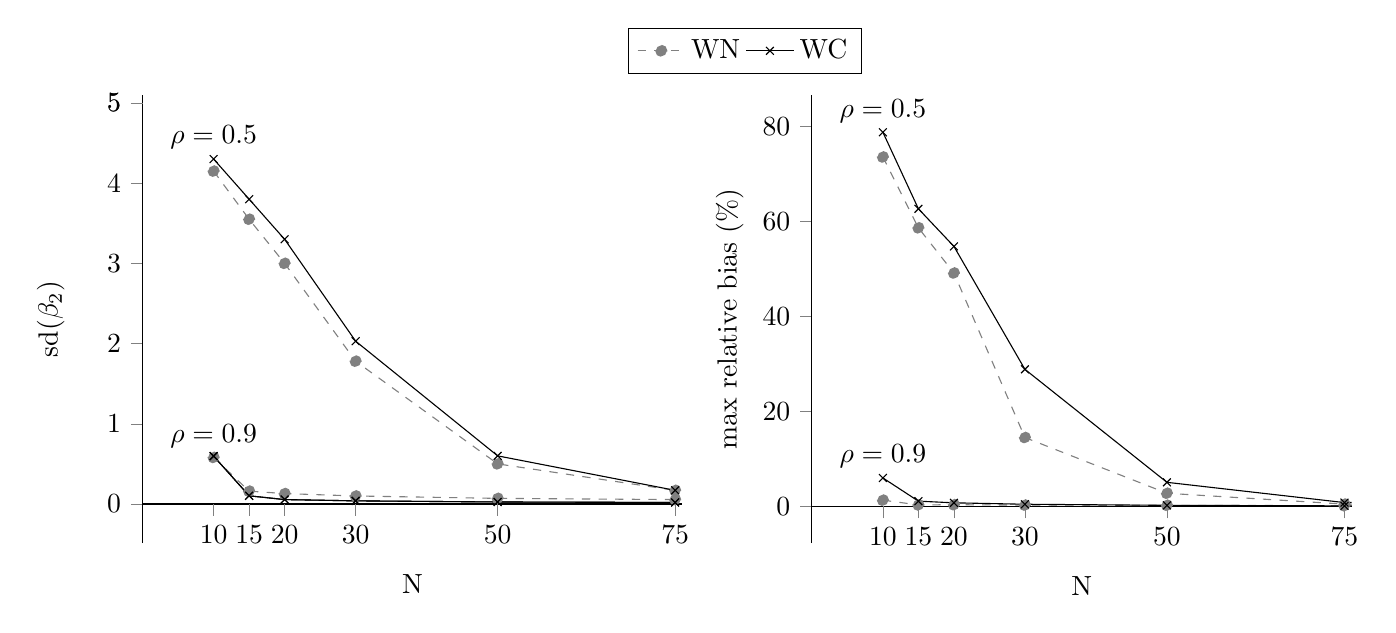
\begin{tikzpicture}[
	scale=1,
	]	
	
	%WN sds
	\begin{axis}[
	axis on top=true,
	%xshift= 6cm,
	scale=1,
	%width=15cm,
	axis x line*=middle , axis y line*=left,
	xtick=\empty,
	%ytick=\empty,
	extra y ticks = {5},
	%extra y tick labels = {0.02, 0.05,0.07, 0.10, 0.14},
	ytick align = outside,
	xtick align = outside,
	xlabel = {N},
	ylabel = sd($\beta_2$),
	extra x ticks = {10, 15, 20, 30, 50, 75,100},
	xlabel near ticks,
    ymax=5.1,
	xmin=0, xmax=76,
	legend style ={at={(0.90,1.15)}, 
		anchor=north west, draw=black, 
		fill=white, legend columns=-1}]
	

	\addplot[mark=*, color=gray, dashed]    coordinates {(10,0.58)(15, 0.16)(20, 0.13)(30,0.10)(50,0.07)(75,0.055) %(100,0)
	} node[pos=0] (rho) {};
	\node [above] at (rho) {$\rho=0.9$}; %rho=0.9
	\addlegendentry{WN};
	\addplot[mark=x, color=black]   coordinates {(10,0.597)(15, 0.102)(20, 0.055)(30,0.039)(50,0.025)(75,0.019) %(100,0.016)
	};  
	\addlegendentry{WC};
	
	\addplot[mark=*, color=gray, dashed]    coordinates {(10,4.15)(15, 3.55)(20, 3.00)(30,1.78)(50,0.50)(75,0.17) %(100,0)
	}; 
	\addplot[mark=x, color=black]   coordinates {(10,4.3)(15, 3.8)(20, 3.3)(30,2.03)(50,0.60)(75,0.17) %(100,0.12)
	} node[pos=0] (rho) {};
	\node [above] at (rho) {$\rho=0.5$}; %rho=0.5
	
	\addplot[mark=x, color=black]   coordinates {(10,0.597)(15, 0.102)(20, 0.055)(30,0.039)(50,0.025)(75,0.019) %(100,0.016)
	};  

	
\end{axis}
	
\begin{axis}[
	axis on top=true,
	xshift= 8.5cm,
	scale=1,
	%width=15cm,
	axis x line*=middle , axis y line*=left,
	xtick=\empty,
	%ytick=\empty,
	%extra y ticks = {0.02, 0.05, 0.07, 0.1, 0.14},
	%extra y tick labels = {0.02, 0.05,0.07, 0.10, 0.14},
	ytick align = outside,
	xtick align = outside,
	xlabel = {N},
	ylabel = max relative bias (\%),
	extra x ticks = {10, 15, 20, 30, 50, 75,100},
	xlabel near ticks,
	%ymin=0, ymax=2.0,
	xmin=0, xmax=76]
	

	\addplot[mark=*, color=gray, dashed]    coordinates {(10,1.33)(15, 0.33)(20, 0.37)(30,0.29)(50,0.25)(75,0.16)(100,0)}; %rho=0.9 WN
		
	\addplot[mark=*, color=gray, dashed]    coordinates {(10,73.5)(15,58.6)(20, 49.1)(30,14.5)(50,2.78)(75,0.5)(100,0)}; %rho=0.5 WN
	
	\addplot[mark=x, color=black]   coordinates {(10,6.0)(15, 1.12)(20, 0.77)(30,0.47)(50,0.24)(75,0.13)(100,0.1)} node[pos=0] (rho) {};
	\node [above] at (rho) {$\rho=0.9$}; %rho=0.9WC
	
	\addplot[mark=x, color=black]   coordinates {(10,78.7)(15,62.6)(20, 54.7)(30,28.84)(50,5.08)(75,0.82)(100,1.16)} node[pos=0] (rho) {};
	\node [above] at (rho) {$\rho=0.5$}; %rho=0.5 WC
	
	\end{axis}
	
	\end{tikzpicture}  
\end{document}